\documentclass[11 pt]{article}
\usepackage{graphicx}
%\usepackage{mysty}
%\usepackage{amsmath}
\usepackage{url}

\begin{document}

\section*{Computerized Resonance Experiments}

Build a resonance system using available resources.
Using LabVIEW or Python, sweep through drive frequencies and measure the amplitude and phase response of the system.

\subsection*{Too-Simple Example}

Connect two Vernier GoDirect Sensor Carts (i.e. 204A carts) with three springs and the SinDrive device:

driver --spring-- cart 1 --spring-- cart 2 --spring-- track endstop.

Write a Python program that sweeps through an appropriate range of drive frequencies and uses the Vernier GoDirect Python library to measure cart position/time data at that frequency. 
Use the numpy.fft library to calculate the amplitude and phase of the cart motion, relative to the drive phase.
Use this data to make a plot such as figure \ref{fig:2-carts}.

\begin{figure}[h]
	\begin{center}
		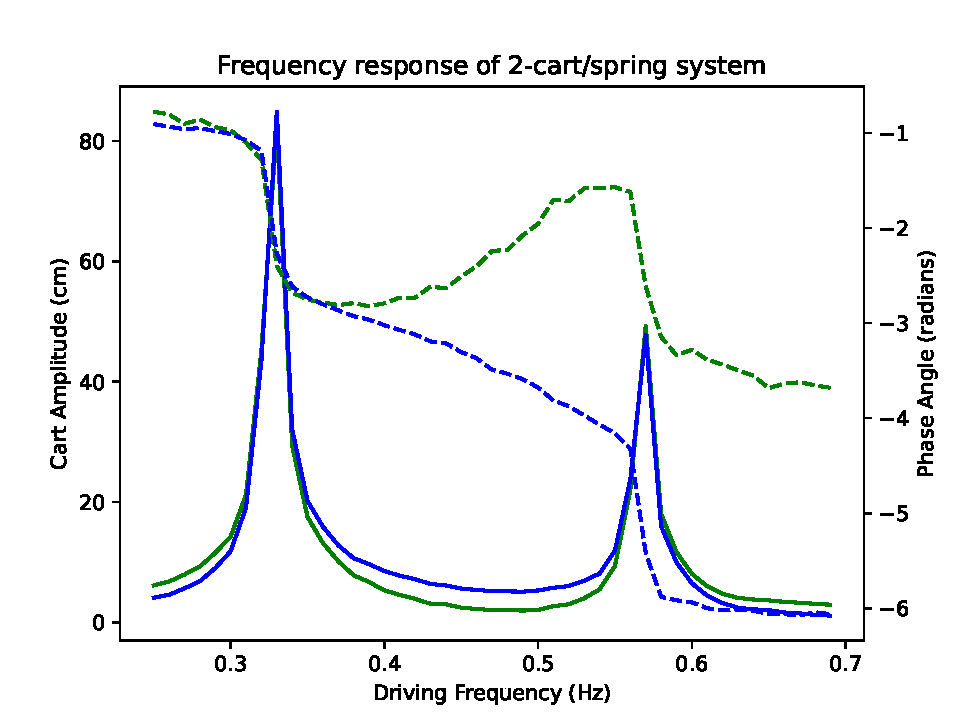
\includegraphics{2-cart_response}
	\end{center}
	\caption{Amplitude(solid lines) and phase (dashed lines) for two coupled carts}
	\label{fig:2-carts}
\end{figure}

\subsection*{Resources}
\begin{itemize}
	\item Dr. Ayars's CartDriver library: \url{https://github.com/EricAyars/Cart-driver}
		This library (located in the `Control' folder of that repository) provides a simple object-oriented API for controlling everything about the SinDrive apparatus.
		Example usage is included in CartDriver.py
	\item Vernier Software provides an API for all of their GoDirect sensors, including carts:\url{https://www.vernier.com/engineering/python/}. You will need to install the godirect library on your python installation (pip install godirect). 
		Once that's done, it's easiest to use the godirect library from within the 
\end{itemize}<++>

\end{document}

